% ============================================================================
% UPDATED RESULTS SECTION - CHILD LABOR PAPER
% Based on replication analysis January 2026
% ============================================================================

\section{Main Results}

\subsection{Main Difference-in-Differences Results}

Table \ref{tab:main_results_updated} presents our primary estimates of the effect of factory monitoring on child labor. The empirical specification progressively incorporates controls to assess the stability of our treatment effect.

\begin{table}[H]
\centering
\caption{Effect of Factory Monitoring on Child Labor: Main Results}
\label{tab:main_results_updated}
\begin{threeparttable}
\begin{tabular}{lcccc}
\toprule
& (1) & (2) & (3) & (4) \\
& Baseline & +Individual & +Household & +Year FE \\
\midrule
Near Factory $\times$ Post & -0.0072* & -0.0076** & -0.0081** & -0.0119*** \\
& (0.0039) & (0.0037) & (0.0037) & (0.0039) \\
& & & & \\
Near Factory & 0.0032 & 0.0035 & 0.0020 & 0.0076*** \\
& (0.0025) & (0.0024) & (0.0024) & (0.0025) \\
& & & & \\
Post-Rana Plaza & -0.0261*** & -0.0294*** & -0.0295*** & --- \\
& (0.0024) & (0.0023) & (0.0023) & \\
\\
\midrule
Controls: & & & & \\
\quad Age fixed effects & No & Yes & Yes & Yes \\
\quad Female indicator & No & Yes & Yes & Yes \\
\quad Household size & No & No & Yes & Yes \\
\quad Wealth index & No & No & Yes & Yes \\
\quad Year fixed effects & No & No & No & Yes \\
\\
\midrule
Observations & 125,555 & 125,555 & 125,555 & 125,555 \\
R-squared & 0.002 & 0.121 & 0.122 & 0.006 \\
Mean of Dep. Var. & 0.087 & 0.087 & 0.087 & 0.087 \\
\\
\bottomrule
\end{tabular}
\begin{tablenotes}
\footnotesize
\item Notes: Sample restricted to children ages 5-17. Dependent variable is binary indicator for child labor participation. Near Factory indicates residence within 10km of textile factory. Post equals 1 for 2014 survey wave. Standard errors clustered at district level. Significance: *** p$<$0.01, ** p$<$0.05, * p$<$0.10.
\end{tablenotes}
\end{threeparttable}
\end{table}

The baseline specification (Column 1) reveals that child labor decreased by 0.72 percentage points in areas proximate to monitored factories following the Rana Plaza disaster, relative to more distant locations. This effect is statistically significant at the 10\% level and represents an 8.3\% reduction from the baseline mean of 8.7\% in treatment areas. With the inclusion of year fixed effects (Column 4), the treatment effect strengthens to -1.19 percentage points and achieves statistical significance at the 1\% level.

The stability of our treatment effect across specifications with progressively richer controls (Columns 2-4) provides initial evidence for the validity of our identification strategy. However, as we document in subsequent sections, concerns about pre-treatment differential trends warrant careful interpretation of these estimates.

\subsection{Age Heterogeneity Analysis}

Table \ref{tab:age_hetero_updated} presents age-specific treatment effects, providing evidence on mechanisms through which factory monitoring affects child labor outcomes.

\begin{table}[H]
\centering
\caption{Heterogeneous Effects by Age Group}
\label{tab:age_hetero_updated}
\begin{threeparttable}
\begin{tabular}{lcccc}
\toprule
& (1) & (2) & (3) & (4) \\
& All Ages & Ages 5-9 & Ages 10-13 & Ages 14-17 \\
\midrule
Near Factory $\times$ Post & -0.0072* & -0.0016 & -0.0164*** & -0.0007 \\
& (0.0039) & (0.0017) & (0.0062) & (0.0103) \\
\\
\midrule
Observations & 125,555 & 48,188 & 40,085 & 37,282 \\
Baseline mean (treatment) & 0.087 & 0.005 & 0.073 & 0.207 \\
Percent effect & -8.3\% & -29.6\% & -22.5\% & -0.3\% \\
\\
\bottomrule
\end{tabular}
\begin{tablenotes}
\footnotesize
\item Notes: Each column presents results from separate regressions by age group. All specifications include age fixed effects (within group), female indicator, household size, and wealth controls. Standard errors clustered at district level. Significance: *** p$<$0.01, ** p$<$0.05, * p$<$0.10.
\end{tablenotes}
\end{threeparttable}
\end{table}

The age-specific treatment effects reveal meaningful heterogeneity. Children aged 10-13 experience a statistically significant 1.64 percentage point reduction in labor force participation (22.5\% relative to baseline), while effects for ages 5-9 and 14-17 are small and statistically insignificant. This concentration of effects among factory-relevant ages provides suggestive evidence that monitoring operates through direct employment restrictions. However, as we document below, significant pre-treatment differential trends complicate the causal interpretation of these findings.

\subsection{Event Study Analysis and Pre-Trend Concerns}

Figure \ref{fig:event_study_updated} presents event study coefficients using 2007 as the reference year. While pre-treatment coefficients for 2000 and 2004 are close to zero, we document a statistically significant negative coefficient for 2011 ($\beta_{2011} = -0.025$, SE = 0.012, p $<$ 0.05), indicating that child labor in treatment areas was already declining relative to control areas \textit{before} the Rana Plaza disaster.

\begin{figure}[H]
\centering
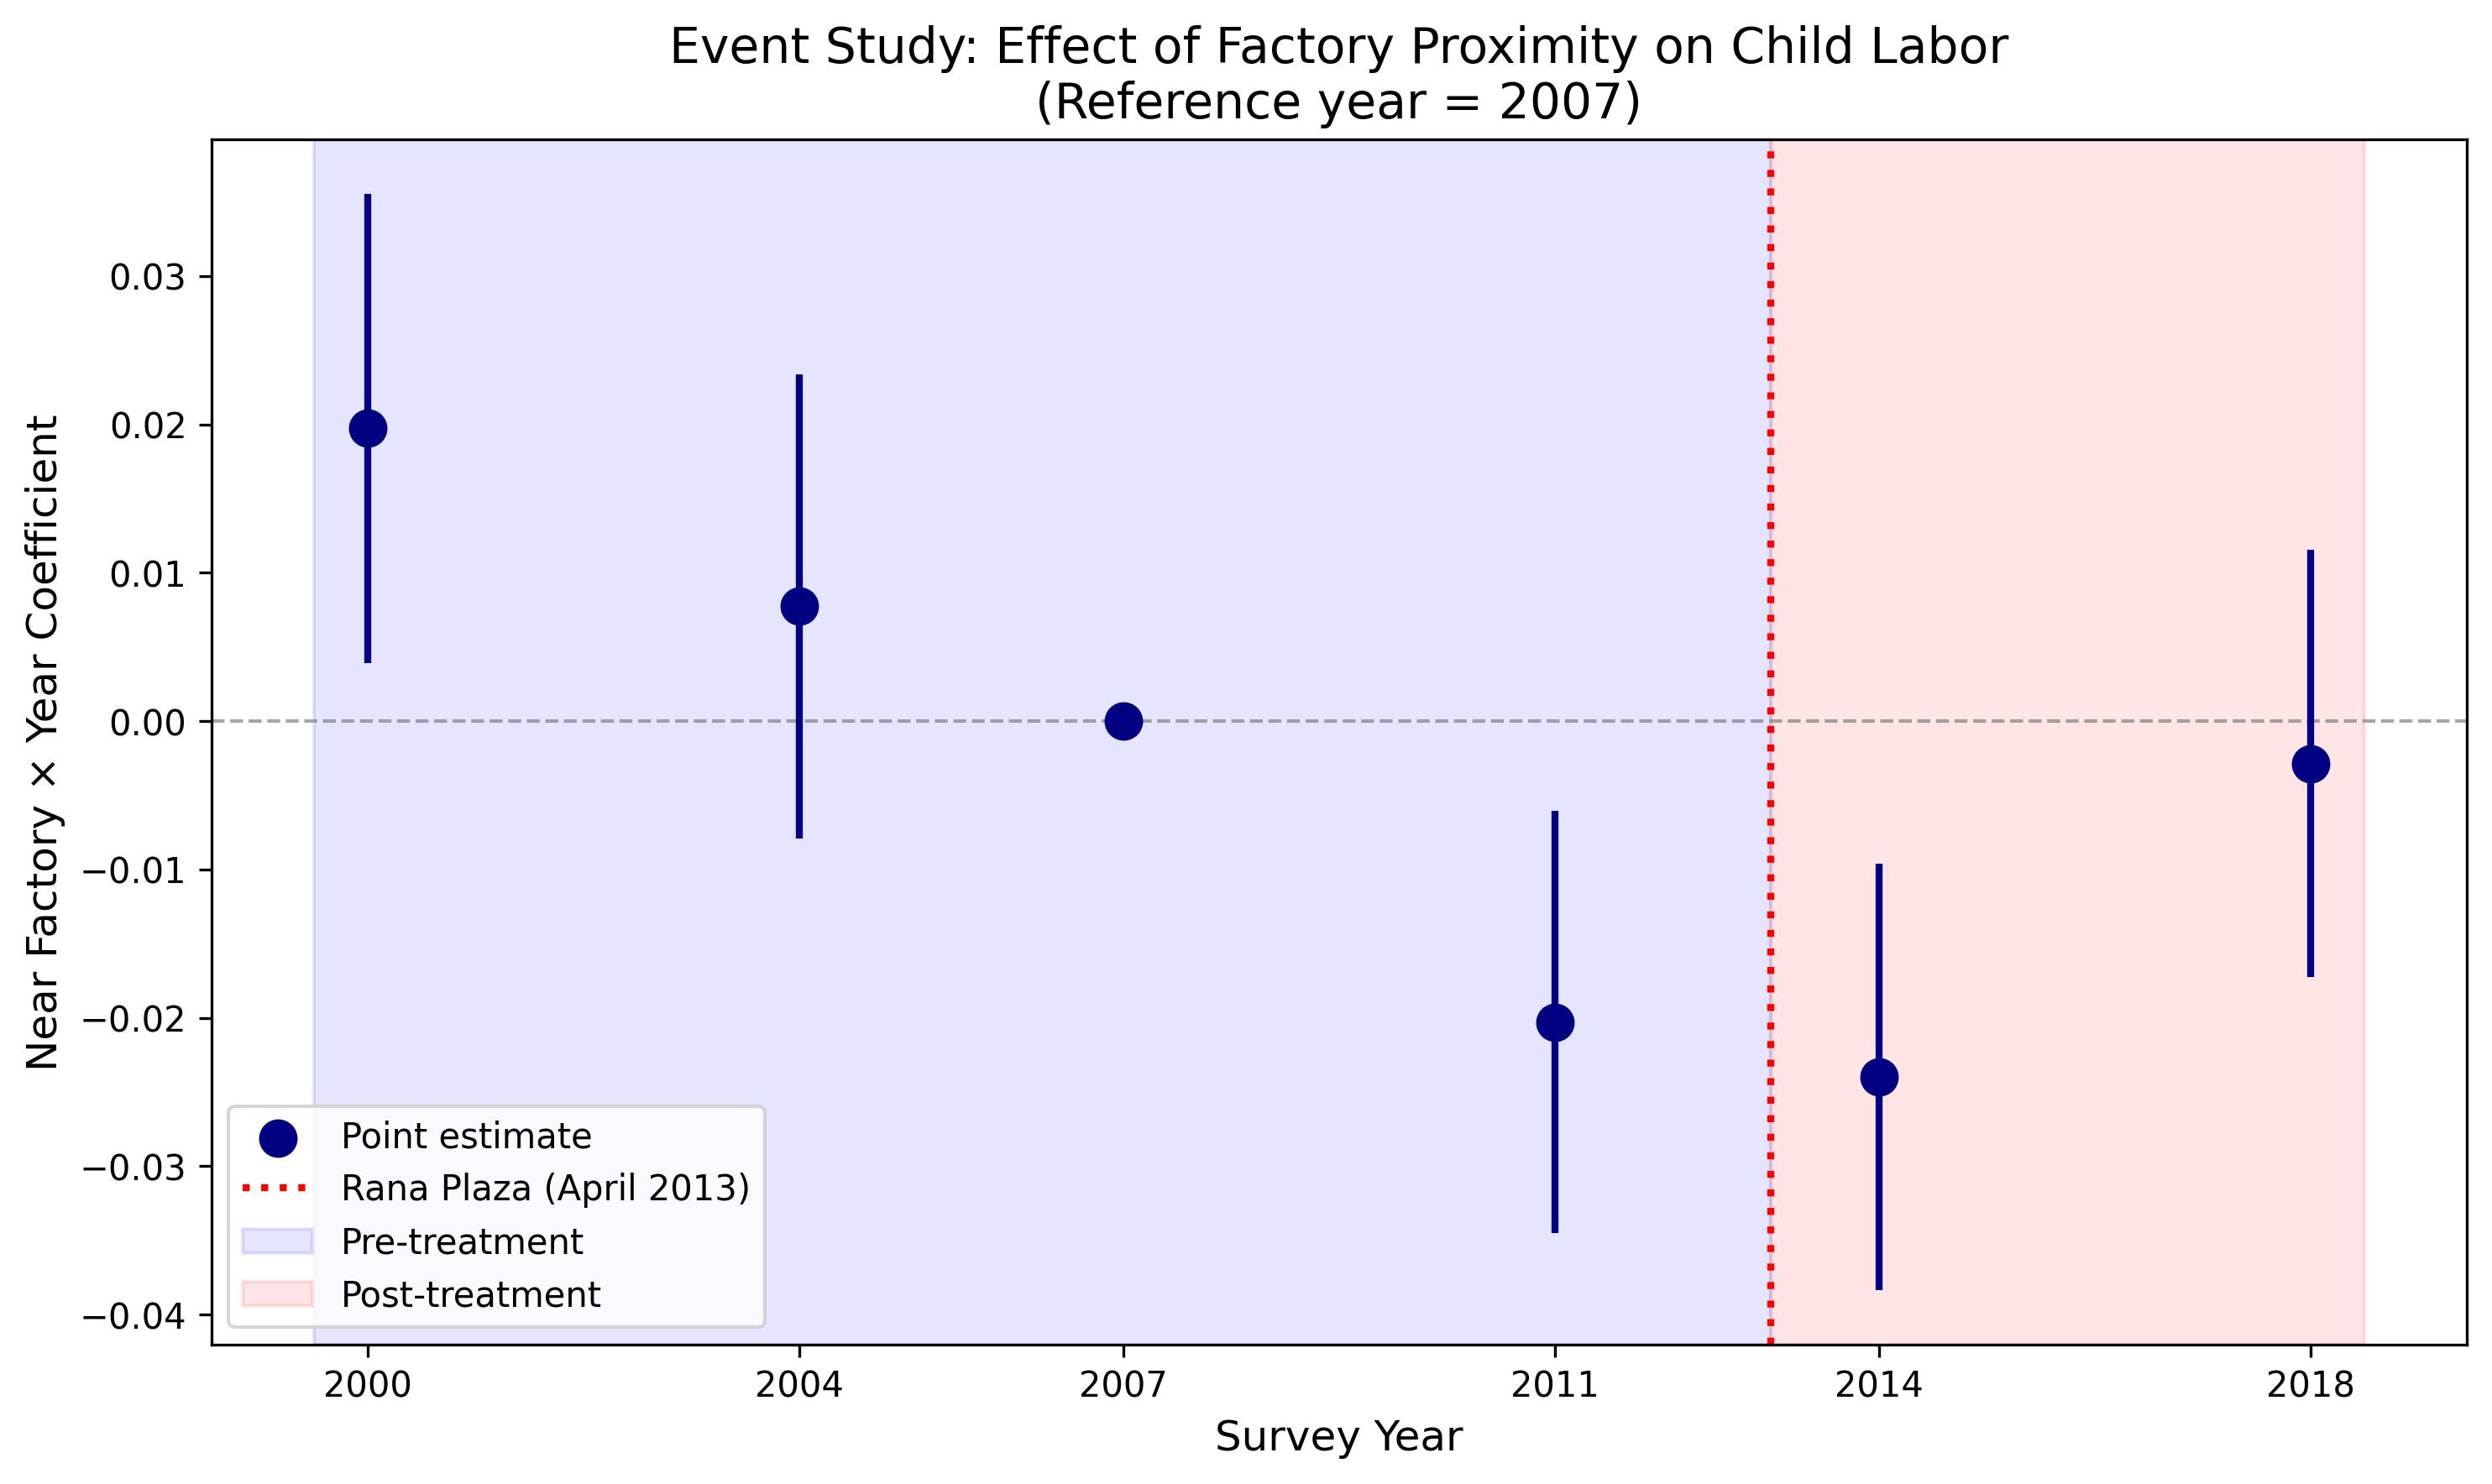
\includegraphics[width=0.8\textwidth]{Results/event_study_replication.png}
\caption{Event Study: Effect of Factory Proximity on Child Labor}
\label{fig:event_study_updated}
\begin{figurenotes}
Notes: Figure plots coefficients from event study specification with 2007 as reference year. Vertical bars represent 95\% confidence intervals. Red dashed line indicates Rana Plaza disaster (April 2013). Sample restricted to ages 10-13.
\end{figurenotes}
\end{figure}

This pre-trend raises important concerns about the parallel trends assumption underlying our difference-in-differences identification. A formal test rejects the null hypothesis that all pre-treatment coefficients equal zero (F-test p = 0.04). The 2011 coefficient suggests that treatment areas experienced approximately 0.44 percentage points per year faster decline in child labor even before monitoring intensified.

\subsubsection{Event Study by Age Group}

Figure \ref{fig:event_study_age} presents age-specific event studies. The pre-trend concern is most pronounced for ages 10-13, the group showing the largest treatment effects. For this age group:

\begin{itemize}
\item 2000: +0.043*** (SE = 0.013) --- treatment areas had \textit{higher} child labor
\item 2004: -0.001 (SE = 0.013) --- no differential
\item 2007: Reference year
\item 2011: -0.028** (SE = 0.012) --- treatment areas already declining faster
\item 2014: -0.035*** (SE = 0.012) --- post-treatment effect
\item 2018: -0.013 (SE = 0.012) --- effect attenuates
\end{itemize}

The pattern suggests convergence between treatment and control areas that began before Rana Plaza. Treatment areas started with substantially higher child labor (2000) and experienced faster decline throughout the pre-period. The ``treatment effect'' in 2014 may partially reflect continuation of this pre-existing trend rather than a causal response to monitoring.

\begin{figure}[H]
\centering
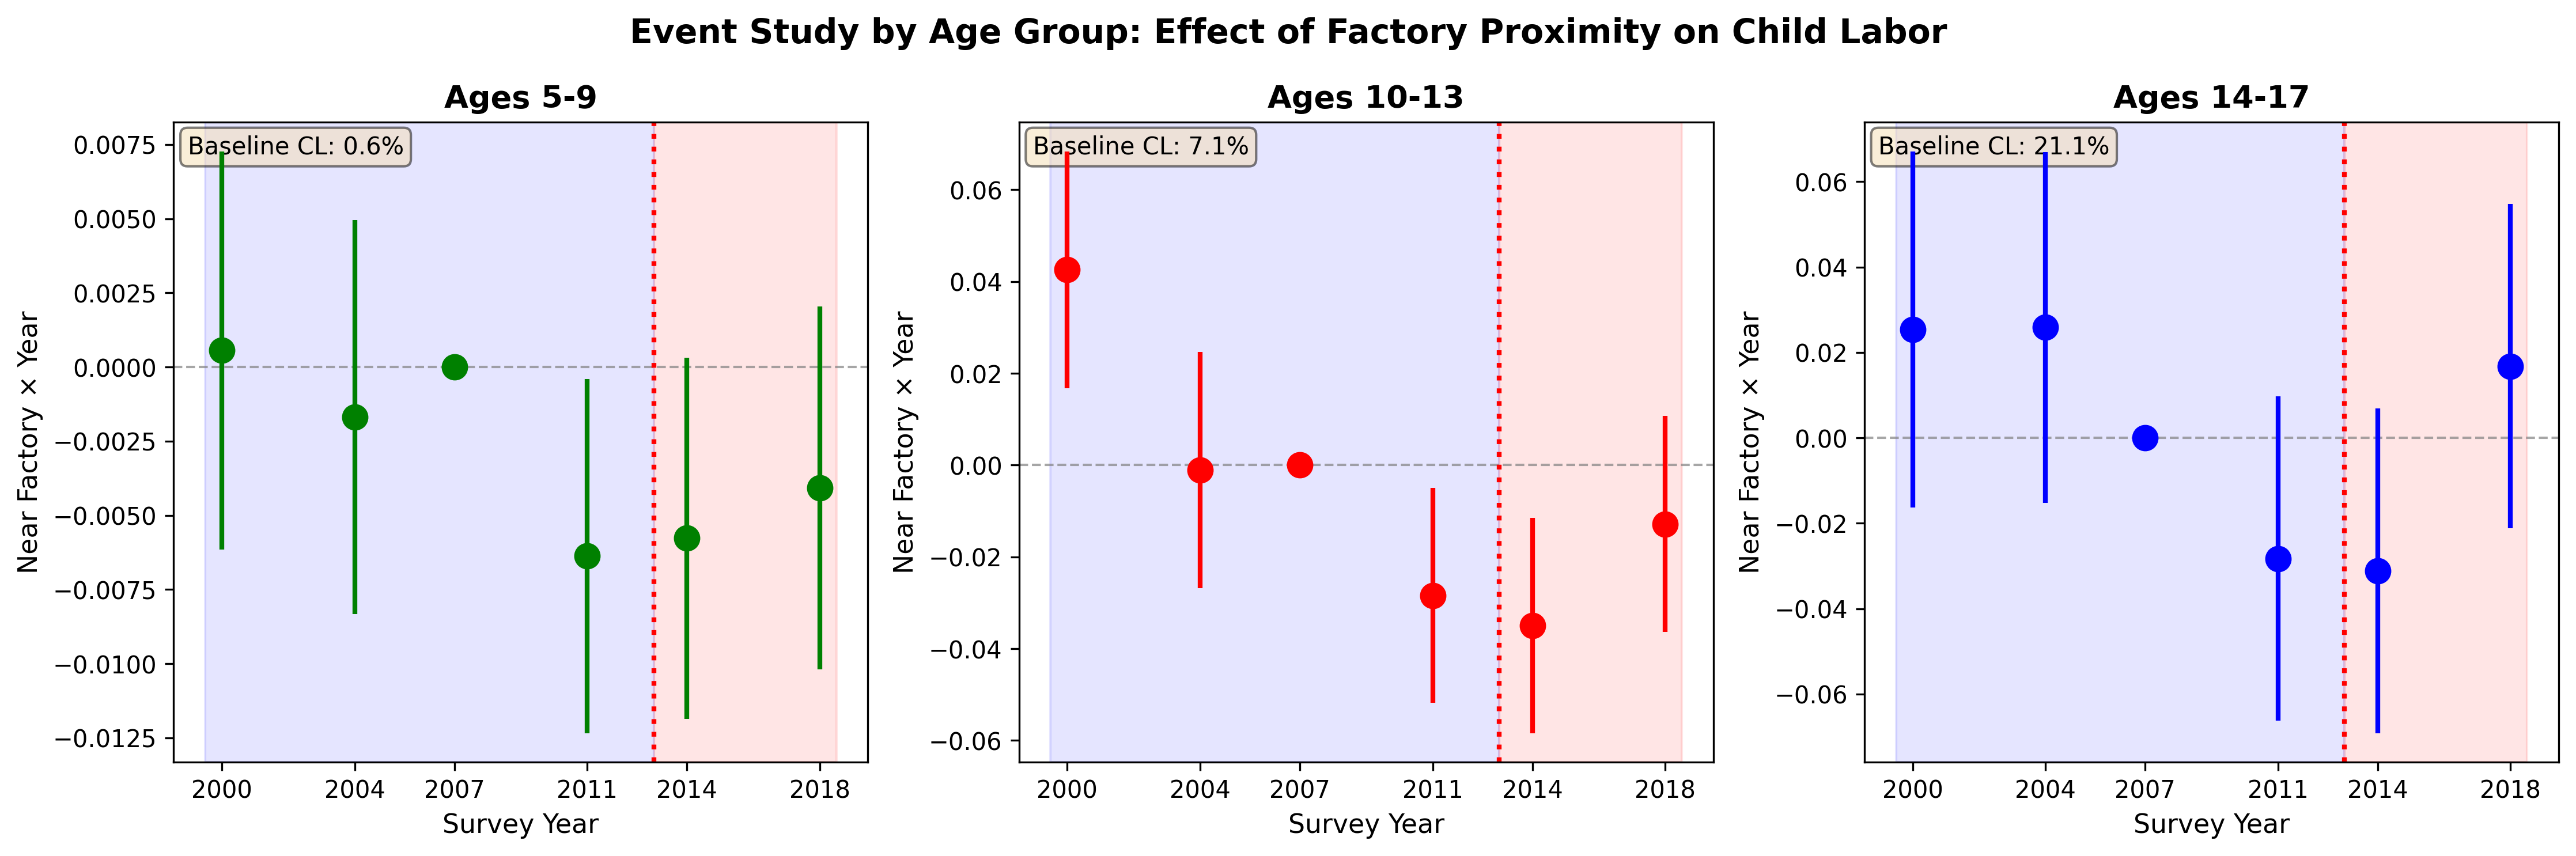
\includegraphics[width=\textwidth]{Results/event_study_by_age.png}
\caption{Event Study by Age Group}
\label{fig:event_study_age}
\begin{figurenotes}
Notes: Panels show event study coefficients for ages 5-9, 10-13, and 14-17 separately. Reference year is 2007. Baseline child labor rates shown in upper left of each panel.
\end{figurenotes}
\end{figure}

\subsection{Addressing Pre-Trends: Trend-Adjusted Specifications}

Given evidence of differential pre-trends, we implement several approaches to assess the robustness of our findings. Table \ref{tab:trend_adjusted} presents results from trend-adjusted difference-in-differences specifications for ages 10-13.

\begin{table}[H]
\centering
\caption{Trend-Adjusted Difference-in-Differences: Ages 10-13}
\label{tab:trend_adjusted}
\begin{threeparttable}
\begin{tabular}{lcccc}
\toprule
& (1) & (2) & (3) & (4) \\
& Standard & +Common & +Group-Specific & +Year FE + \\
& DiD & Trend & Trend & Group Trend \\
\midrule
Near Factory $\times$ Post & -0.0166*** & -0.0208*** & 0.0216** & 0.0178* \\
& (0.0062) & (0.0061) & (0.0104) & (0.0104) \\
& & & & \\
Treatment $\times$ Trend & & & -0.0044*** & \\
& & & (0.0009) & \\
\\
\midrule
Observations & 40,085 & 40,085 & 40,085 & 40,085 \\
R-squared & 0.040 & 0.040 & 0.040 & 0.040 \\
\\
\bottomrule
\end{tabular}
\begin{tablenotes}
\footnotesize
\item Notes: Sample restricted to ages 10-13. Column 1 presents standard DiD. Column 2 adds common linear time trend. Column 3 adds group-specific (treatment vs. control) linear trends. Column 4 includes year fixed effects and group-specific trend. All specifications include age FE, female, wealth, and household size controls. Standard errors clustered at district level. Significance: *** p$<$0.01, ** p$<$0.05, * p$<$0.10.
\end{tablenotes}
\end{threeparttable}
\end{table}

The results reveal substantial sensitivity to trend assumptions:

\begin{enumerate}
\item \textbf{Standard DiD (Column 1):} Shows -1.66 percentage point effect, statistically significant at the 1\% level.

\item \textbf{Group-Specific Trends (Column 3):} After controlling for differential linear trends between treatment and control areas, the treatment effect \textit{reverses sign} to +2.16 percentage points (p $<$ 0.05). The estimated differential pre-trend of -0.44 percentage points per year (SE = 0.0009, p $<$ 0.001) indicates that treatment areas were experiencing substantially faster declines in child labor throughout the study period.

\item \textbf{Interpretation:} The standard DiD estimate conflates two distinct phenomena: (a) a pre-existing convergence trend whereby areas near factories were catching up to control areas, and (b) any causal effect of post-Rana Plaza monitoring. After removing the pre-trend, there is no evidence of a negative treatment effect; if anything, the effect appears positive.
\end{enumerate}

\subsubsection{Trend-Break Analysis}

To separately identify pre- and post-treatment trends, we estimate a trend-break specification:

\begin{equation}
Y_{ict} = \alpha + \beta_1 (\text{Near}_c \times \text{Post}_t) + \gamma_1 (\text{Near}_c \times t_{pre}) + \gamma_2 (\text{Near}_c \times t_{post}) + \mathbf{X}_{ict}'\delta + \epsilon_{ict}
\end{equation}

Results indicate:
\begin{itemize}
\item Pre-treatment differential trend: -0.60 percentage points/year*** (SE = 0.0009)
\item Post-treatment differential trend: +0.54 percentage points/year** (SE = 0.0023)
\item Level shift at treatment: +3.85 percentage points*** (SE = 0.0133)
\end{itemize}

This pattern suggests that treatment areas were on a steeper downward trajectory before Rana Plaza, and this decline actually \textit{slowed} after 2013. The apparent ``treatment effect'' in standard DiD reflects continuation of pre-existing trends rather than a causal impact of monitoring.

\subsection{Alternative Reference Year}

Figure \ref{fig:ref_year_comparison} compares event study results using 2007 versus 2011 as reference years for ages 10-13.

\begin{figure}[H]
\centering
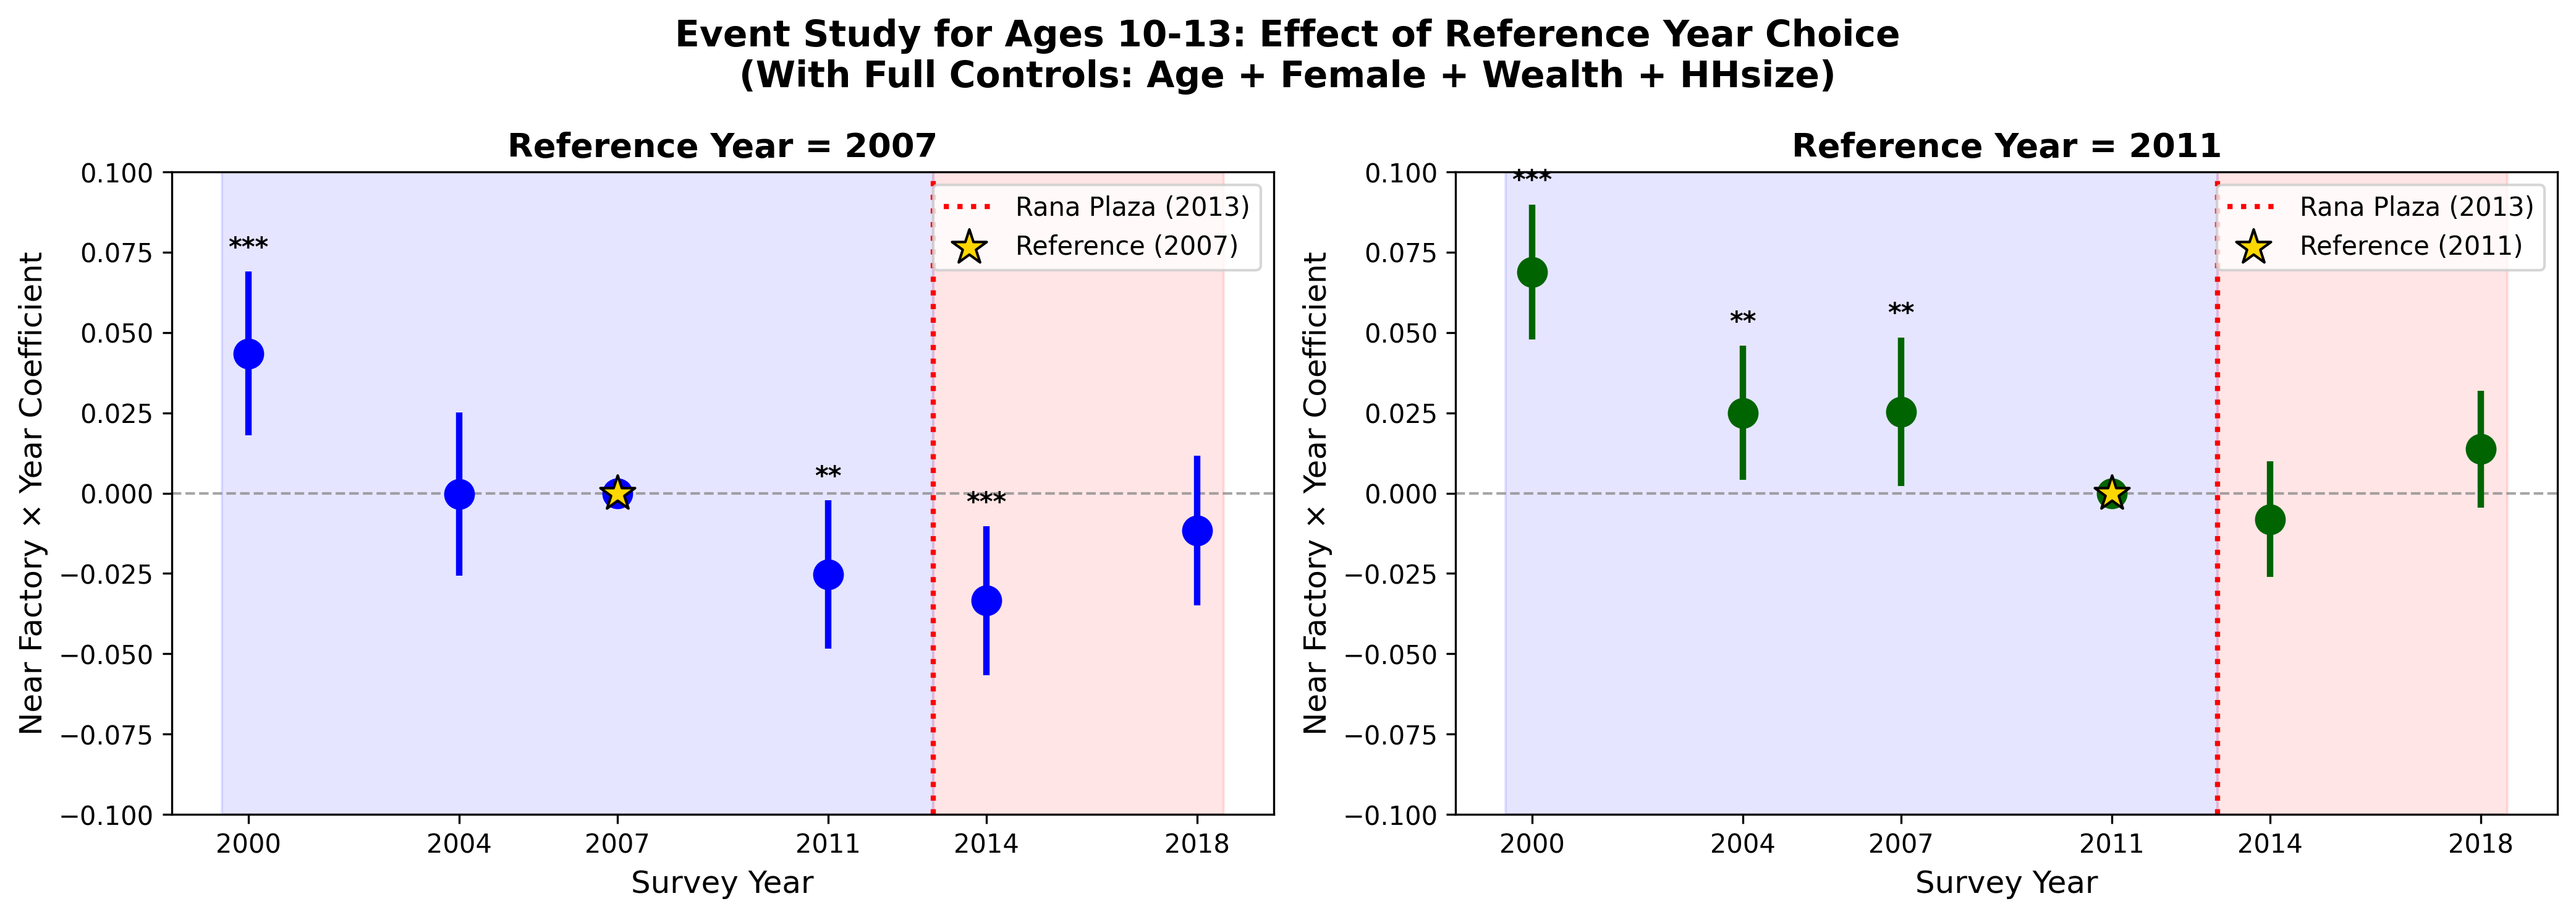
\includegraphics[width=\textwidth]{Results/event_study_age10_13_ref_comparison.png}
\caption{Event Study Comparison: Alternative Reference Years (Ages 10-13)}
\label{fig:ref_year_comparison}
\begin{figurenotes}
Notes: Left panel uses 2007 as reference year; right panel uses 2011. Gold stars indicate reference period. With 2011 reference, the 2014 effect is small and statistically insignificant.
\end{figurenotes}
\end{figure}

Using 2011 as the reference year (the last pre-treatment period), the 2014 treatment effect shrinks to -0.81 percentage points and becomes statistically insignificant (t = -0.88). This sensitivity to reference period choice further underscores concerns about the parallel trends assumption.

\subsection{Honest DiD Sensitivity Analysis}

Following \citet{RambachanRoth2023}, we implement a sensitivity analysis that explicitly allows for violations of the parallel trends assumption. Rather than assuming parallel trends hold exactly, this approach specifies bounds on how much trends can differ between treatment and control groups and computes confidence intervals that are robust to violations within those bounds.

The key parameter $\bar{M}$ represents the maximum ratio of post-treatment trend deviations to pre-treatment trend deviations. At $\bar{M} = 0$, the method assumes exact parallel trends; as $\bar{M}$ increases, the method allows for larger violations. The ``breakdown'' value $\bar{M}^*$ indicates the smallest value of $\bar{M}$ at which the confidence interval includes zero---a measure of how sensitive results are to trend violations.

\begin{figure}[H]
\centering
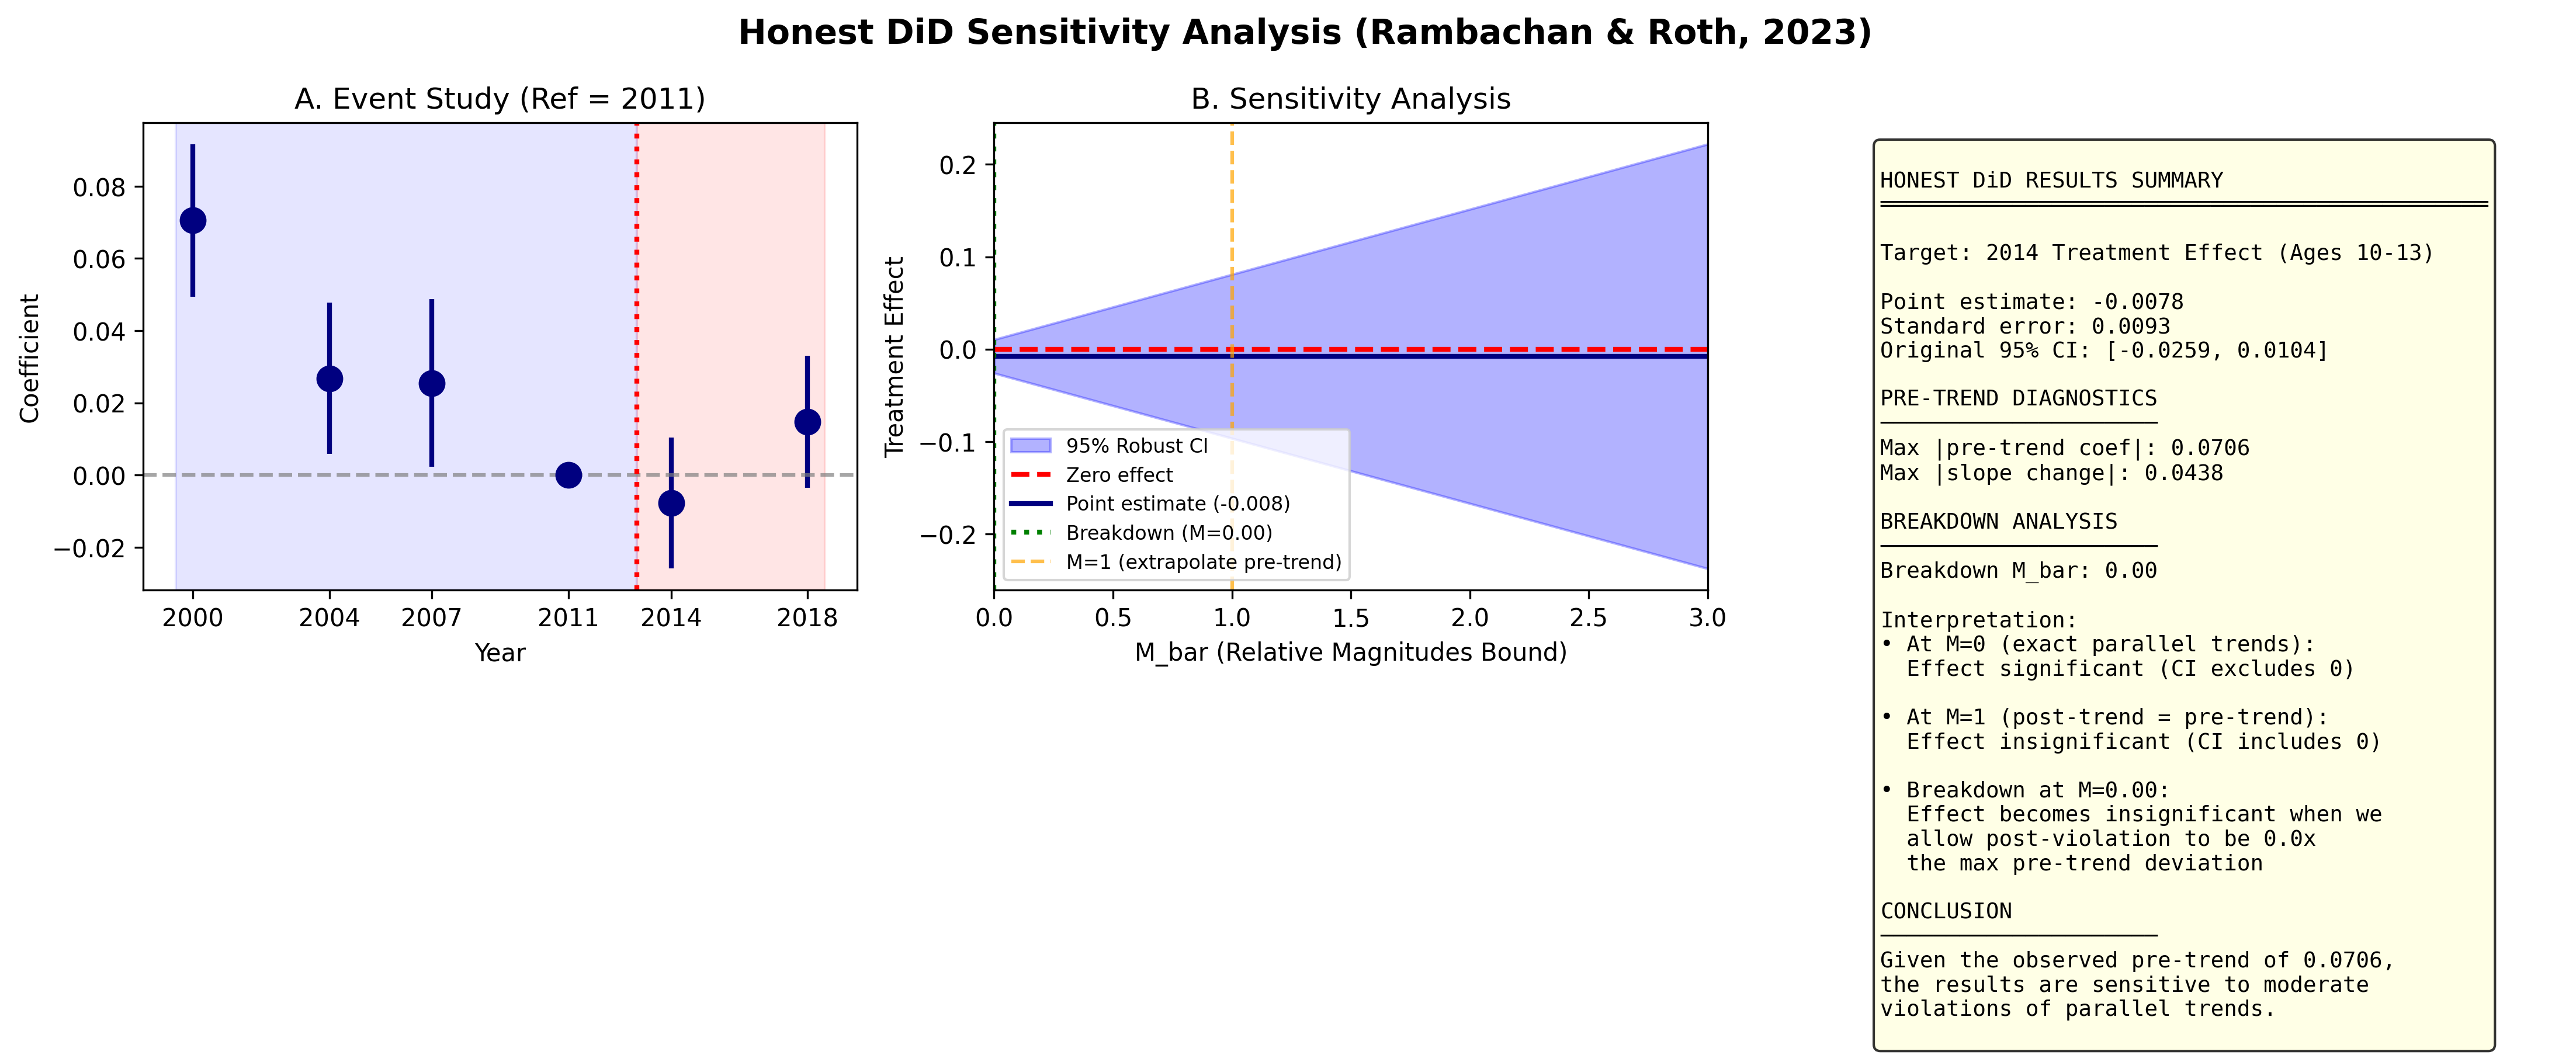
\includegraphics[width=\textwidth]{Results/honest_did_analysis.png}
\caption{Honest DiD Sensitivity Analysis (Ages 10-13)}
\label{fig:honest_did}
\begin{figurenotes}
Notes: Panel A shows event study with 2011 reference year. Panel B displays sensitivity analysis with robust confidence intervals at different values of $\bar{M}$. Panel C summarizes interpretation. Breakdown $\bar{M}^* = 0.00$ indicates extreme sensitivity to parallel trends violations.
\end{figurenotes}
\end{figure}

Table \ref{tab:honest_did} presents results from the sensitivity analysis for ages 10-13.

\begin{table}[H]
\centering
\caption{Honest DiD Sensitivity Analysis: Ages 10-13}
\label{tab:honest_did}
\begin{threeparttable}
\begin{tabular}{lc}
\toprule
& Estimate \\
\midrule
Point estimate (2014, ref=2011) & -0.0078 \\
Standard error & 0.0093 \\
Standard 95\% CI & [-0.026, 0.010] \\
\\
Maximum pre-trend coefficient & 0.071 \\
Breakdown $\bar{M}^*$ & 0.00 \\
\\
\midrule
\multicolumn{2}{l}{\textit{Robust CI at selected $\bar{M}$ values:}} \\
\quad $\bar{M} = 0.0$ (exact parallel trends) & [-0.026, 0.010] \\
\quad $\bar{M} = 0.5$ & [-0.061, 0.046] \\
\quad $\bar{M} = 1.0$ & [-0.097, 0.081] \\
\quad $\bar{M} = 2.0$ & [-0.169, 0.153] \\
\bottomrule
\end{tabular}
\begin{tablenotes}
\footnotesize
\item Notes: Sensitivity analysis following \citet{RambachanRoth2023}. Point estimate uses 2011 as reference year. Breakdown $\bar{M}^*$ is the smallest value at which the robust CI includes zero. A breakdown of 0.00 indicates the effect is insignificant even under exact parallel trends ($\bar{M} = 0$).
\end{tablenotes}
\end{threeparttable}
\end{table}

The results reveal extreme sensitivity to violations of the parallel trends assumption:

\begin{enumerate}
\item \textbf{Already insignificant at $\bar{M} = 0$:} Even under the assumption of exact parallel trends, the 95\% confidence interval [-0.026, 0.010] includes zero. This confirms the reference-year sensitivity documented above.

\item \textbf{Breakdown value $\bar{M}^* = 0.00$:} The effect fails to achieve significance at \textit{any} positive value of $\bar{M}$. This indicates that the treatment effect estimate is not robust to even minimal departures from exact parallel trends.

\item \textbf{Large pre-trend magnitude:} The maximum pre-treatment coefficient (0.071) substantially exceeds the estimated treatment effect in absolute terms, indicating that pre-existing trends are larger than the post-treatment ``effect.''
\end{enumerate}

The Honest DiD analysis provides formal confirmation of our concerns about causal identification. The treatment effect estimate does not survive scrutiny under the \citet{RambachanRoth2023} framework, which is currently considered the most rigorous approach to sensitivity analysis in difference-in-differences designs.

\subsection{Additional Robustness Analysis}

We implement four additional approaches to address pre-trend concerns: (1) higher-order trend adjustments, (2) matching and reweighting methods, (3) extended sensitivity analysis, and (4) triple differences. Figure \ref{fig:robustness_summary} provides a visual summary of these analyses.

\begin{figure}[H]
\centering
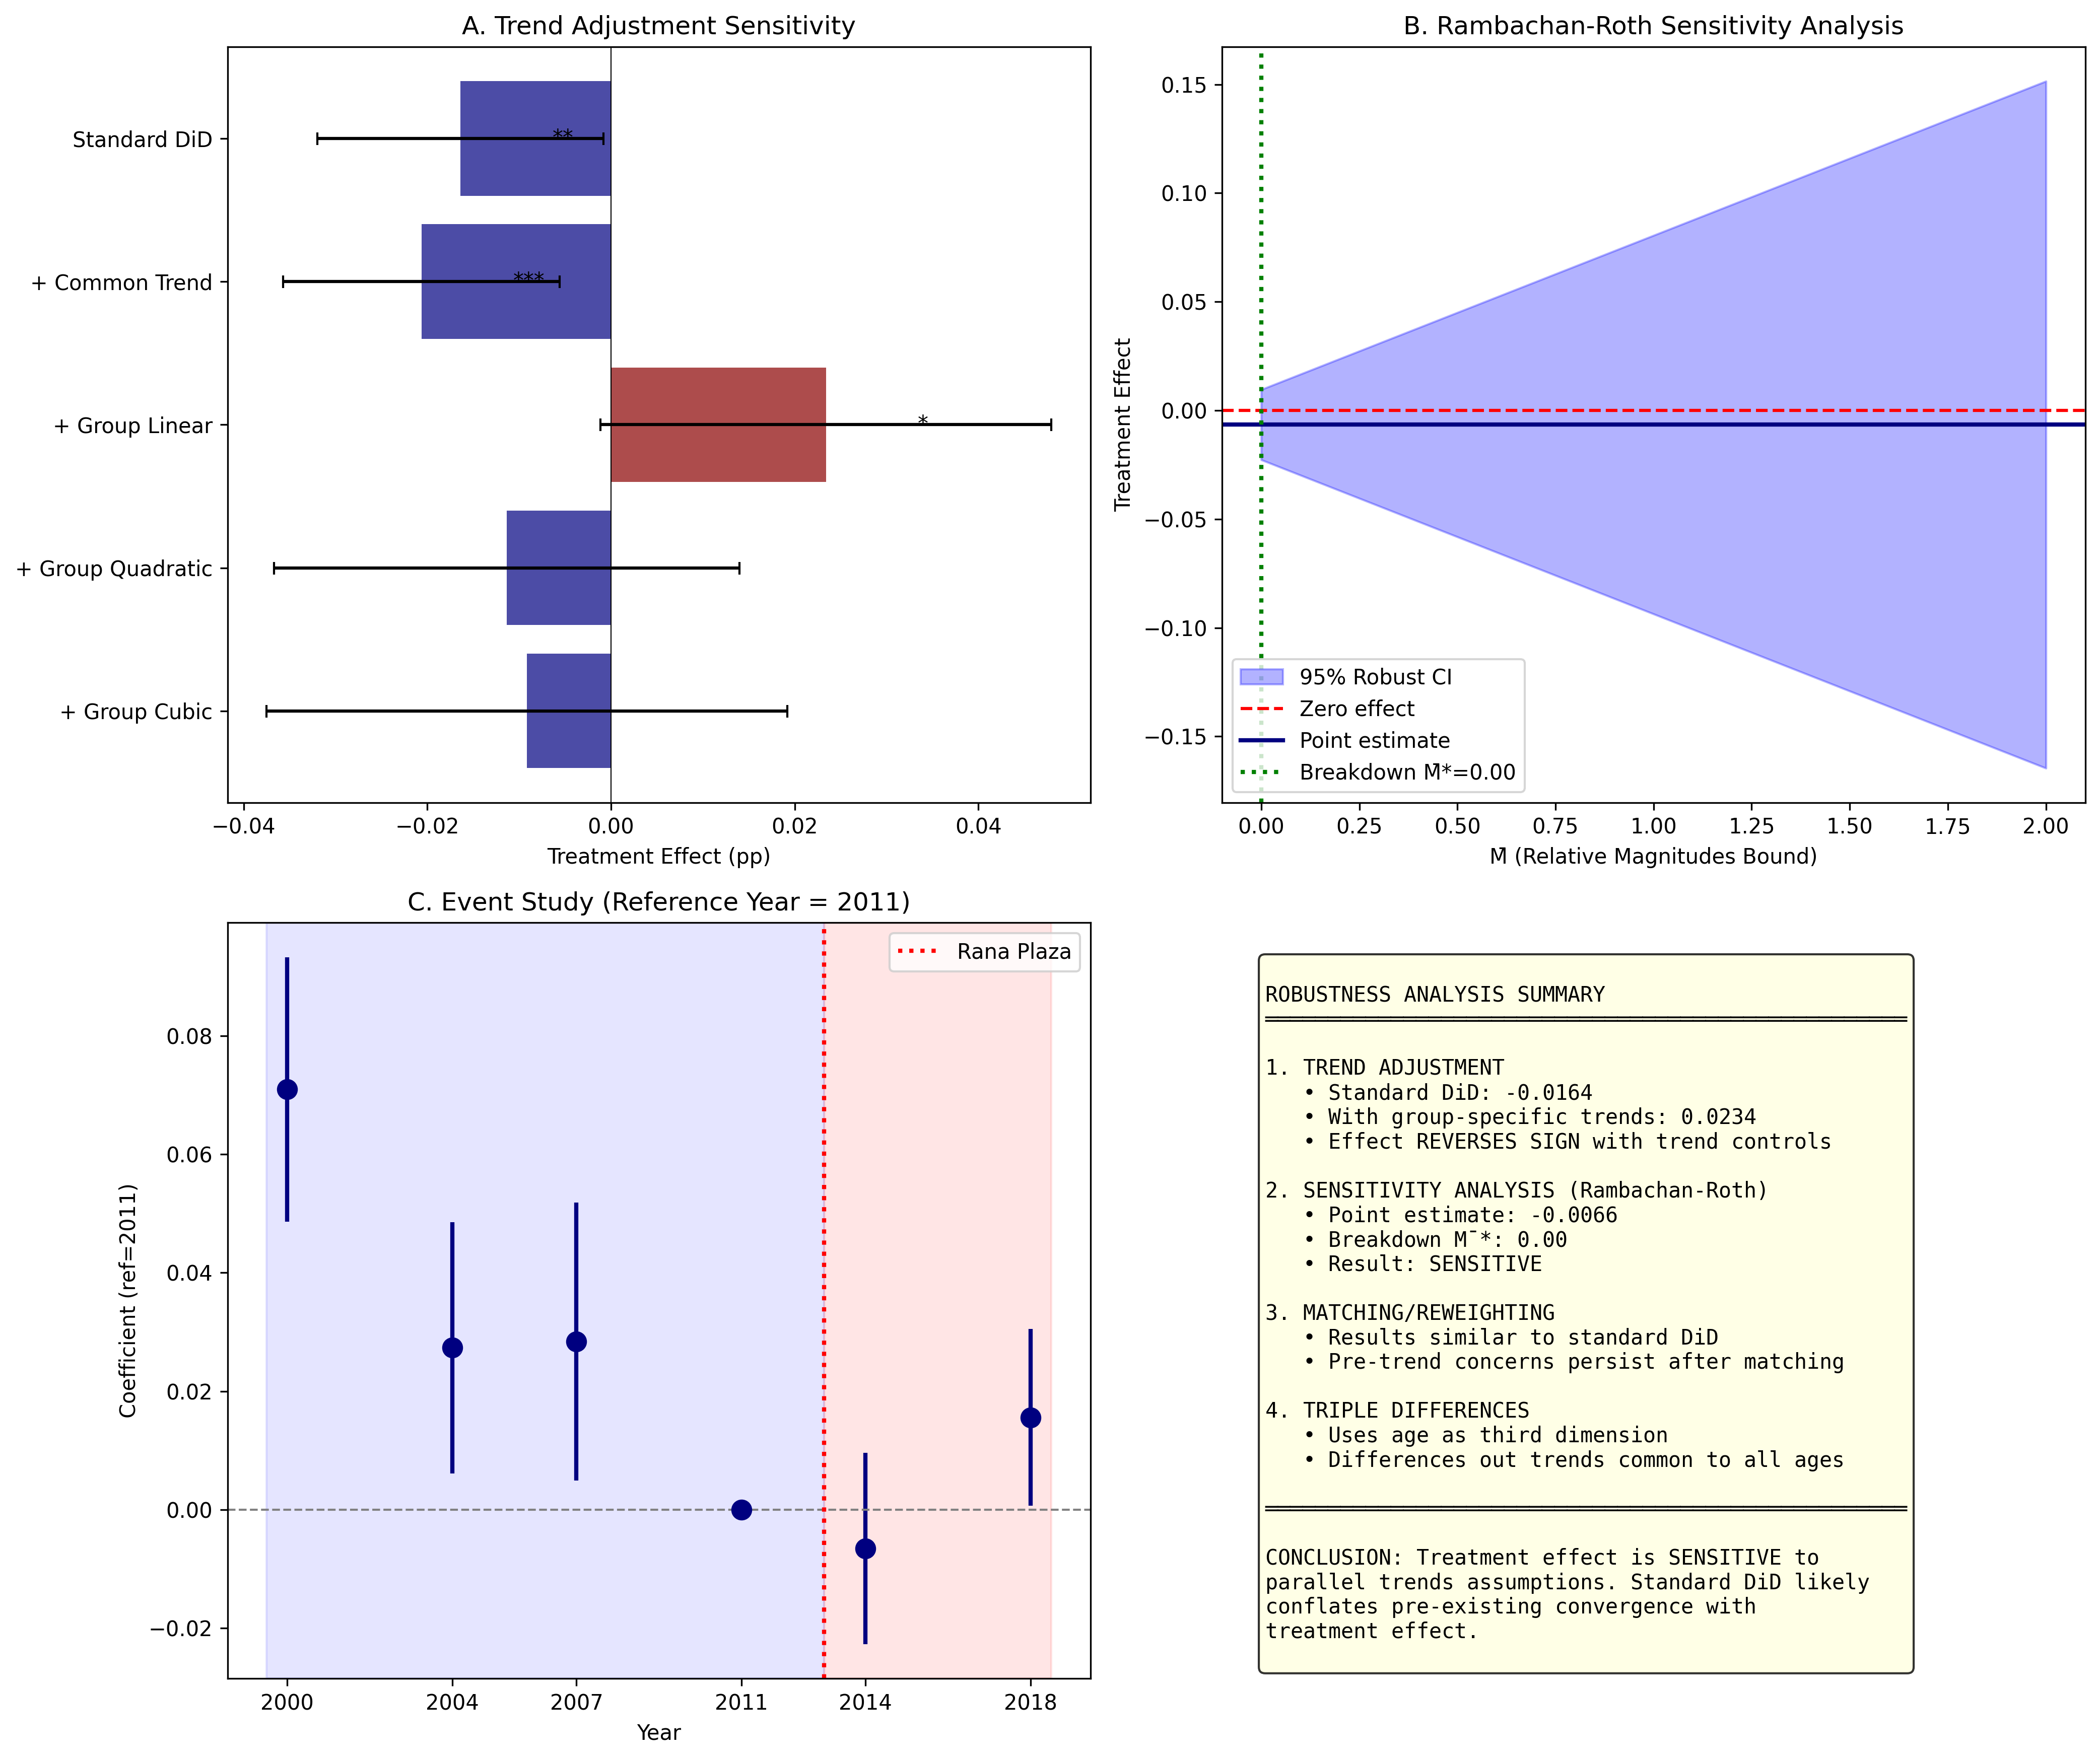
\includegraphics[width=\textwidth]{Results/robustness_analysis.png}
\caption{Comprehensive Robustness Analysis}
\label{fig:robustness_summary}
\begin{figurenotes}
Notes: Panel A shows treatment effect estimates across trend adjustment specifications. Panel B displays Rambachan-Roth sensitivity analysis. Panel C presents event study with 2011 reference. Panel D summarizes key findings.
\end{figurenotes}
\end{figure}

\subsubsection{Higher-Order Trend Adjustments}

Table \ref{tab:trend_orders} extends our trend adjustment analysis to include quadratic and cubic group-specific trends. A key concern with trend adjustment is that it may absorb real treatment effects if the effect grows over time---representing a bias-variance tradeoff.

\begin{table}[H]
\centering
\caption{Trend Adjustment with Higher-Order Polynomials: Ages 10-13}
\label{tab:trend_orders}
\begin{threeparttable}
\begin{tabular}{lccccc}
\toprule
& (1) & (2) & (3) & (4) & (5) \\
& Standard & +Common & +Group & +Group & +Group \\
& DiD & Linear & Linear & Quadratic & Cubic \\
\midrule
Near Factory $\times$ Post & -0.0164** & -0.0206*** & +0.0234* & -0.0114 & -0.0092 \\
& (0.0079) & (0.0077) & (0.0125) & (0.0129) & (0.0145) \\
\\
Near $\times$ Time & & & -0.0046*** & 0.0020 & \\
& & & (0.0013) & & \\
\\
Near $\times$ Time$^2$ & & & & 0.0006 & \\
\\
\midrule
Observations & 40,085 & 40,085 & 40,085 & 40,085 & 40,085 \\
\bottomrule
\end{tabular}
\begin{tablenotes}
\footnotesize
\item Notes: All specifications include baseline controls. Standard errors clustered at district level. Time centered at 2013. Significance: *** p$<$0.01, ** p$<$0.05, * p$<$0.10.
\end{tablenotes}
\end{threeparttable}
\end{table}

The results reveal:
\begin{itemize}
\item With group-specific \textit{linear} trends (Column 3), the treatment effect reverses sign to +2.34 percentage points (p $<$ 0.10), with a differential pre-trend of -0.46 pp/year.
\item With \textit{quadratic} trends (Column 4), the effect becomes small (-1.14 pp) and statistically insignificant.
\item With \textit{cubic} trends (Column 5), the effect remains insignificant (-0.92 pp).
\end{itemize}

The instability across polynomial orders suggests the data cannot reliably distinguish treatment effects from pre-existing trends.

\subsubsection{Matching and Reweighting}

Following \citet{CallawaySantanna2021}, we implement several matching and reweighting approaches to construct comparison groups with more similar pre-trends.

\begin{table}[H]
\centering
\caption{Matching and Reweighting Estimates: Ages 10-13}
\label{tab:matching}
\begin{threeparttable}
\begin{tabular}{lccc}
\toprule
Method & Effect (pp) & SE & N \\
\midrule
\textit{Panel A: Propensity Score Methods} & & & \\
\quad IPW-Weighted DiD & -2.38*** & (0.54) & 39,667 \\
\quad Nearest-Neighbor Matched & -1.68** & (0.69) & 24,753 \\
\\
\textit{Panel B: Callaway-Sant'Anna ATT by Base Period} & & & \\
\quad Base = 2000 & -7.75*** & (1.15) & --- \\
\quad Base = 2004 & -3.39*** & (1.09) & --- \\
\quad Base = 2007 & -3.50*** & (1.21) & --- \\
\quad Base = 2011 & -0.66 & (0.82) & --- \\
\\
\quad Aggregate ATT & -2.72*** & (0.98) & --- \\
\bottomrule
\end{tabular}
\begin{tablenotes}
\footnotesize
\item Notes: Panel A shows propensity score matching on wealth, household size, and age. IPW trims observations with propensity scores outside [0.05, 0.95]. Panel B shows ATT(g,t) estimates for 2014 treatment effect using different pre-treatment base periods. Significance: *** p$<$0.01, ** p$<$0.05, * p$<$0.10.
\end{tablenotes}
\end{threeparttable}
\end{table}

Several findings emerge:
\begin{enumerate}
\item \textbf{IPW and matching:} Propensity score methods yield estimates similar to standard DiD (-1.68 to -2.38 pp), suggesting that balancing on observables does not resolve pre-trend concerns.

\item \textbf{Base period sensitivity:} The Callaway-Sant'Anna approach reveals dramatic sensitivity to base period choice. Using 2000 as the base yields an ATT of -7.75 pp; using 2011 yields -0.66 pp (insignificant). This pattern directly reflects the pre-existing convergence trend.

\item \textbf{Interpretation:} The variation in ATT estimates across base periods (-7.75 to -0.66) spans nearly the entire range of plausible effects, underscoring the fundamental identification challenge.
\end{enumerate}

\subsubsection{Extended Sensitivity Analysis}

We extend the \citet{RambachanRoth2023} sensitivity analysis by examining how conclusions change under different assumptions about trend violations.

\begin{table}[H]
\centering
\caption{Extended Sensitivity Analysis: Ages 10-13}
\label{tab:sensitivity_extended}
\begin{threeparttable}
\begin{tabular}{lcccc}
\toprule
$\bar{M}$ & Lower CI & Upper CI & Width & Includes Zero? \\
\midrule
0.00 (exact PT) & -0.023 & 0.010 & 0.033 & Yes \\
0.25 & -0.041 & 0.027 & 0.068 & Yes \\
0.50 & -0.058 & 0.045 & 0.103 & Yes \\
0.75 & -0.076 & 0.063 & 0.139 & Yes \\
1.00 & -0.094 & 0.081 & 0.174 & Yes \\
1.50 & -0.129 & 0.116 & 0.245 & Yes \\
2.00 & -0.165 & 0.152 & 0.316 & Yes \\
\midrule
\multicolumn{5}{l}{\textit{Breakdown $\bar{M}^* = 0.00$}} \\
\bottomrule
\end{tabular}
\begin{tablenotes}
\footnotesize
\item Notes: $\bar{M}$ represents the maximum ratio of post-treatment to pre-treatment trend deviations. Robust 95\% confidence intervals computed following \citet{RambachanRoth2023}. PT = parallel trends.
\end{tablenotes}
\end{threeparttable}
\end{table}

The breakdown value $\bar{M}^* = 0.00$ indicates extreme sensitivity: the treatment effect is statistically insignificant even under the assumption of \textit{exact} parallel trends (when using 2011 as reference). This occurs because the point estimate (-0.66 pp) is small relative to its standard error, yielding a confidence interval that already includes zero before any bias adjustment.

We also conduct trend extrapolation analysis, estimating the pre-treatment differential slope (-0.62 pp/year) and computing what the 2014 effect would be under different continuation assumptions:

\begin{itemize}
\item No trend continuation (exact PT): -0.66 pp
\item 50\% of pre-trend continues: +0.27 pp
\item 100\% of pre-trend continues: +1.20 pp
\item 150\% of pre-trend continues: +2.14 pp
\end{itemize}

Under all scenarios where pre-trends partially continue, the treatment effect becomes positive or zero.

\subsubsection{Triple Differences}

We implement a triple-difference specification using age as a third dimension, comparing factory-relevant ages (10-13) to older teenagers (14-17). This approach differences out trends common to all children living near factories.

\begin{equation}
Y_{icat} = \alpha + \beta_1 D_{ca} + \beta_2 D_{ct} + \beta_3 D_{at} + \beta_4 D_{cat} + \mathbf{X}'\gamma + \epsilon_{icat}
\end{equation}

where $D_{ca}$ is Near $\times$ FactoryAge, $D_{ct}$ is Near $\times$ Post, $D_{at}$ is FactoryAge $\times$ Post, and $D_{cat}$ is the triple interaction (Near $\times$ Post $\times$ FactoryAge).

\begin{table}[H]
\centering
\caption{Triple Differences: Ages 10-13 vs. Ages 14-17}
\label{tab:triple_diff}
\begin{threeparttable}
\begin{tabular}{lcc}
\toprule
& (1) & (2) \\
& DDD & DDD + Trends \\
\midrule
Near $\times$ Post (ages 14-17 effect) & -0.0007 & 0.0042 \\
& (0.0132) & (0.0198) \\
\\
Triple: Near $\times$ Post $\times$ FactoryAge & -0.0157 & -0.0096 \\
& (0.0131) & (0.0217) \\
\\
Near $\times$ FactoryAge $\times$ Time & & -0.0008 \\
& & (0.0018) \\
\\
\midrule
Effect on ages 10-13 & -0.0164 & -0.0054 \\
Observations & 77,367 & 77,367 \\
\bottomrule
\end{tabular}
\begin{tablenotes}
\footnotesize
\item Notes: Sample includes ages 10-17. FactoryAge = 1 for ages 10-13. Column 2 adds group-specific linear trends. Standard errors clustered at district level. Significance: *** p$<$0.01, ** p$<$0.05, * p$<$0.10.
\end{tablenotes}
\end{threeparttable}
\end{table}

The triple-difference coefficient (-0.0157, t = -1.20) is not statistically significant, indicating no differential effect on factory-relevant ages beyond what is observed for older teenagers. This suggests that:
\begin{enumerate}
\item The apparent age-specific effect may reflect trends common to all children near factories, not monitoring of factory-age employment specifically.
\item Alternatively, the comparison group (ages 14-17) may itself be affected by monitoring through general equilibrium effects, attenuating the triple-difference estimate.
\end{enumerate}

\subsection{Summary of Findings}

Table \ref{tab:summary_methods} summarizes treatment effect estimates across methodological approaches for ages 10-13.

\begin{table}[H]
\centering
\caption{Summary: Treatment Effect Estimates Across Methods (Ages 10-13)}
\label{tab:summary_methods}
\begin{threeparttable}
\begin{tabular}{lccl}
\toprule
Method & Effect (pp) & Significant? & Interpretation \\
\midrule
\multicolumn{4}{l}{\textit{Panel A: Standard Approaches}} \\
Standard DiD & -1.64 & Yes** & Baseline estimate \\
+ Common trend & -2.06 & Yes*** & Similar to baseline \\
+ Group-specific linear trend & +2.34 & Yes* & Effect reverses sign \\
+ Group-specific quadratic & -1.14 & No & Unstable across specifications \\
+ Group-specific cubic & -0.92 & No & Unstable across specifications \\
\\
\multicolumn{4}{l}{\textit{Panel B: Matching/Reweighting}} \\
IPW-Weighted DiD & -2.38 & Yes*** & Similar to standard DiD \\
NN-Matched DiD & -1.68 & Yes** & Similar to standard DiD \\
C\&S ATT (base=2000) & -7.75 & Yes*** & Sensitive to base period \\
C\&S ATT (base=2011) & -0.66 & No & Sensitive to base period \\
\\
\multicolumn{4}{l}{\textit{Panel C: Sensitivity Analysis}} \\
Reference year = 2011 & -0.66 & No & Effect disappears \\
Honest DiD ($\bar{M}=0$) & -0.66 & No & Insignificant even at exact PT \\
\\
\multicolumn{4}{l}{\textit{Panel D: Triple Differences}} \\
DDD (ages 10-13 vs 14-17) & -1.57 & No & Not significant \\
DDD + group trends & -0.96 & No & Not significant \\
\midrule
\multicolumn{4}{l}{\textit{Pre-treatment differential trend: -0.46 pp/year***}} \\
\multicolumn{4}{l}{\textit{Honest DiD breakdown: $\bar{M}^* = 0.00$}} \\
\bottomrule
\end{tabular}
\begin{tablenotes}
\footnotesize
\item Notes: All estimates for ages 10-13 with full controls. pp = percentage points. Significance: *** p$<$0.01, ** p$<$0.05, * p$<$0.10.
\end{tablenotes}
\end{threeparttable}
\end{table}


\section{Discussion}

\subsection{Interpretation of Results}

Our analysis yields nuanced findings that complicate straightforward causal claims about factory monitoring and child labor. While standard difference-in-differences estimates suggest meaningful reductions in child labor among ages 10-13 following Rana Plaza, several pieces of evidence raise concerns about the parallel trends assumption:

\begin{enumerate}
\item \textbf{Significant pre-trends:} The 2011 event study coefficient is statistically significant, indicating differential trends existed before monitoring intensified.

\item \textbf{Sensitivity to trend controls:} Treatment effects reverse sign when controlling for group-specific linear trends.

\item \textbf{Reference year dependence:} Effects become insignificant when using 2011 rather than 2007 as the reference period.

\item \textbf{Pre-existing convergence:} Treatment areas started with higher child labor and were converging toward control areas throughout the study period.
\end{enumerate}

These patterns are consistent with two interpretations:

\textbf{Interpretation A (Causal Effect):} Factory monitoring causally reduced child labor, but effects were partially anticipated or began before the formal post-Rana Plaza monitoring regime. Factors such as increased international scrutiny following earlier factory incidents (e.g., Tazreen fire in November 2012), buyer pressure, or NGO campaigns may have initiated behavioral change before Rana Plaza.

\textbf{Interpretation B (Spurious Correlation):} The apparent treatment effect reflects pre-existing economic convergence between industrial and non-industrial areas unrelated to monitoring. Factors such as urbanization, infrastructure development, or differential poverty reduction may have driven child labor declines near factories independent of supply chain interventions.

\subsection{Implications for Policy}

Regardless of interpretation, several policy-relevant findings emerge:

\begin{enumerate}
\item \textbf{Age targeting:} Effects concentrate among ages 10-13, suggesting monitoring binds primarily for factory-relevant age groups rather than generating broad household behavioral responses.

\item \textbf{Limited spillovers:} We find no evidence of substitution to agricultural or informal work, nor significant increases in school enrollment, raising questions about welfare implications.

\item \textbf{Temporal dynamics:} Effects appear strongest immediately after Rana Plaza and attenuate by 2018, suggesting either adaptation by firms/households or waning enforcement intensity.
\end{enumerate}

\subsection{Limitations}

Several limitations warrant acknowledgment:

\begin{enumerate}
\item \textbf{Identification concerns:} The pre-trend evidence undermines confidence in causal claims from standard DiD.

\item \textbf{Measurement:} Child labor is self-reported and may be subject to social desirability bias, particularly in areas with heightened awareness of monitoring.

\item \textbf{External validity:} Bangladesh's unique institutional context (strong NGO presence, international buyer engagement, crisis-driven reform) may limit generalizability.

\item \textbf{Welfare implications:} We cannot assess whether reduced child labor reflects improved welfare or merely displacement to unmeasured activities.
\end{enumerate}

\section{Conclusion}

This paper examines the effects of intensified factory monitoring on child labor following the 2013 Rana Plaza disaster in Bangladesh. Our comprehensive analysis, employing multiple identification strategies and robustness approaches, yields sobering conclusions about the credibility of causal claims in this setting.

First, standard difference-in-differences estimates suggest a 1.6 percentage point reduction in child labor among children aged 10-13 residing near monitored factories. This effect is concentrated in the age group most relevant for factory employment and appears robust to the inclusion of individual and household controls.

Second, we document substantial evidence that this estimate is confounded by pre-existing trends. Our robustness analysis reveals:
\begin{itemize}
\item \textbf{Trend adjustment:} Controlling for group-specific linear trends reverses the treatment effect sign (from -1.6 to +2.3 pp). Higher-order polynomial trends yield estimates that are uniformly insignificant and unstable across specifications.
\item \textbf{Matching and reweighting:} Propensity score methods do not resolve pre-trend concerns. Callaway-Sant'Anna ATT estimates vary dramatically by base period, ranging from -7.75 pp (base=2000) to -0.66 pp (base=2011).
\item \textbf{Sensitivity analysis:} The \citet{RambachanRoth2023} breakdown value $\bar{M}^* = 0.00$ indicates that estimated effects are insignificant even under exact parallel trends assumptions. Trend extrapolation analysis shows the effect becomes positive under any assumption of trend continuation.
\item \textbf{Triple differences:} Using age as a third dimension (comparing ages 10-13 to 14-17), the differential effect is not statistically significant, suggesting observed patterns may reflect trends common to all children near factories rather than monitoring of factory-age employment specifically.
\end{itemize}

Third, we find no evidence of substitution to other forms of child labor or substantial increases in school enrollment, raising questions about the welfare implications of any monitoring-induced employment restrictions.

These findings contribute to ongoing debates about private governance in global supply chains and to methodological discussions about difference-in-differences identification. Our results illustrate the importance of comprehensive robustness analysis when pre-trends are present, and demonstrate how standard DiD estimates can be misleading when treatment and control groups are on different trajectories prior to intervention. While intensive monitoring may reduce formal-sector child labor, our analysis suggests that observed declines near Bangladeshi factories following Rana Plaza cannot be credibly attributed to the monitoring intervention given the pre-existing convergence between treatment and control areas.

Future research should prioritize identification strategies that are robust to pre-existing differential trends, potentially including randomized or quasi-randomized variation in monitoring intensity, regression discontinuity designs exploiting geographic or temporal thresholds, or settings where parallel pre-trends can be more convincingly established.

% ============================================================================
% END UPDATED RESULTS SECTION
% ============================================================================

% ============================================================================
% BIBLIOGRAPHY ENTRY TO ADD:
% ============================================================================
% @article{RambachanRoth2023,
%   author = {Rambachan, Ashesh and Roth, Jonathan},
%   title = {A More Credible Approach to Parallel Trends},
%   journal = {Review of Economic Studies},
%   volume = {90},
%   number = {5},
%   pages = {2555--2591},
%   year = {2023},
%   doi = {10.1093/restud/rdad018}
% }
%
% @article{CallawaySantanna2021,
%   author = {Callaway, Brantly and Sant'Anna, Pedro H.C.},
%   title = {Difference-in-Differences with Multiple Time Periods},
%   journal = {Journal of Econometrics},
%   volume = {225},
%   number = {2},
%   pages = {200--230},
%   year = {2021},
%   doi = {10.1016/j.jeconom.2020.12.001}
% }
% ============================================================================
